\lab{Python}{NumPy Arrays}{NumPy Arrays}
\objective{Create and manipulate powerful NumPy $n$-dimensional arrays.}
\label{lab:NumPyArrays}

\section*{Why Arrays?}
Let's begin with a simple demonstration of why arrays are important for numerical computation.
Why use arrays when Python already has a reasonably efficient list object?
In this demonstration, we will try squaring a matrix.
The matrix will be represented as a two dimensional list (i.e. a list of lists).

The following is a function that will accept two matrices (two dimensional list), $A$ and $B$, and return $AB$ following the usual rules of matrix multiplication.
\lstinputlisting[style=fromfile]{arr_mult.py}
We can initialize a $k \times k$ ``array" of integers like this:
\begin{lstlisting}
>>> k = 10
>>> A = [range(i, i+k) for i in range(0, k**2, k)]
\end{lstlisting}

\begin{problem}
Time how long this function takes to square matrices for increasing values of \li{k}.
In IPython you can time how long it takes for a line of code to execute by prefacing it with \li{\%timeit}, as in \li{\%timeit range(100)}.

Now import NumPy and create a NumPy array, \li{A}, and square it.
\li{A*A} does \emph{not} square the array, but rather multiplies \li{A} with itself element by element.
To get matrix multiplication for NumPy arrays, you must use \li{np.dot} or the \li{dot()} method of an array like this:
\begin{lstlisting}
import numpy as np
A = np.array([range(i, i+k) for i in range(0, k**2, k)])
np.dot(A, A)
\end{lstlisting}
Time how long NumPy takes to square arrays for increasing sizes of \li{k}.
What do you notice about the time needed to square a two dimensional list vs. a two dimensional NumPy array?
\end{problem}

% Below is a comparison of runtimes needed to square a matrix
% \begin{center}
% \begin{tabular}{|c|l|l|}
% \hline
%  Data Structure & Size & Time (s) \\ \hline
%  Python List & $1\times1$ & 0.0000181198 \\ \cline{2-3}
%       & $10\times10$ & 0.0002758503 \\ \cline{2-3}
%       & $100\times100$ & 0.1336028576 \\ \cline{2-3}
%       & $1000\times1000$ & 200.4009799957 \\ \hline \hline
%  NumPy Array & $1\times1$ & 0.0000298023 \\ \cline{2-3}
%       & $10\times10$ & 0.0000109673 \\ \cline{2-3}
%       & $100\times100$ & 0.0009210110 \\ \cline{2-3}
%       & $1000\times1000$ & 2.1682999134 \\ \hline
% \end{tabular}
%
% \end{center}

The reason for the drastic speed difference is that Python, as a high level interpreted language, tends to be slower than lower level compiled languages.
The algorithms implemented in NumPy are heavily optimized and are usually implemented in C or Fortran.
Instead of operating purely in Python, they use Python to run code that is written and optimized in other languages.
NumPy interfaces with some of the best known packages for doing computational linear algebra and can be used to write relatively fast programs.

Lists are still faster for anything that involves a varying lengths of data.
If you are appending to your data or deleting items, consider using lists instead of arrays since both of these operations require the creation of a new array.

\section*{NumPy}
NumPy is one of the fundamental packages for scientific computing with Python.
At its heart lies an efficient $n$-dimensional array, or $ndarray$, object for fast computations.
This lab will focus on how to create and manipulate this powerful object.
These arrays form the foundation of all computations done in NumPy and SciPy (a higher-level scientific computing library built on top of NumPy).
By convention, NumPy is typically imported as
\begin{lstlisting}
>>> import numpy as np
\end{lstlisting}
NumPy also provides a matrix object which is designed to behave like matrices do in MATLAB.
It is strongly encouraged to use NumPy arrays instead of NumPy matrices, despite the latter's convenience.

\section*{Creating Arrays}
The most elementary way to create an array is to define explicitly using \li{np.array()}.
\begin{lstlisting}
>>> a = np.array([1, 3, 5, 7, 11])
>>> a
array([ 1,  3,  5,  7, 11])
\end{lstlisting}
NumPy provides a variety of ways to easily create different kinds of arrays.
\li{np.arange()} creates a ranged array much the same way that Python's \li{range} statement creates a list.
\begin{lstlisting}
>>> b = np.arange(10)
>>> b
array([0, 1, 2, 3, 4, 5, 6, 7, 8, 9])
\end{lstlisting}
We can also create arrays that consist entirely of ones or zeros using \li{np.ones()} and \li{np.zeros()} respectively.
\begin{lstlisting}
>>> c = np.ones(5)
>>> c
array([ 1.,  1.,  1.,  1.,  1.])
>>> d = np.zeros(5)
>>> d
array([ 0.,  0.,  0.,  0.,  0.])
\end{lstlisting}
We can even create an array that has evenly spaced numbers over a desired interval.
The first and second arguments define the endpoints of this closed interval.
\begin{lstlisting}
>>> e = np.linspace(0, 32, num=4)
>>> e
array([  0.        ,  10.66666667,  21.33333333,  32.        ])
\end{lstlisting}
We can even create arrays using random values chosen from a variety of probability distributions.
These functions are stored in a submodule of NumPy, \li{np.random}.
\begin{lstlisting}
>>> f = np.random.rand(5) #uniformly distributed values
>>> f
array([ 0.21845499,  0.73352537,  0.28064456,  0.66878454,  0.44138609])
>>> f = np.random.poisson(1, size=10)
>>> f
array([0, 1, 3, 2, 0, 0, 0, 0, 2, 0])
>>> f = np.random.randn(5) #normally distributed values
array([-1.30752235, -0.60518647,  2.08529266, -0.43919065,  0.92830676])
\end{lstlisting}
We can even allocate an array without initializing its values to any value.
These are useful for when the initial contents of the array are unimportant.
\begin{lstlisting}
>>> g = np.empty(5)
>>> g
array([  0.00000000e+000,   1.30586451e-316,   1.17126324e-316,
         0.00000000e+000,   2.37151510e-322])
\end{lstlisting}

\section*{Array Objects}
NumPy arrays are homogeneous objects.  Unlike Python containers, all of the elements of an array have to be same data type.
Also, unlike Python integers and floats, the data types that NumPy uses in arrays are machine native types.
The benefit of doing this is to avoid the overhead associated with Python's objects.
The result is a tremendous speedup in numerical operations.
NumPy support a variety of types and precision.
\begin{table}
\begin{tabular}{l|l}
Data type & Description \\
\hline
\li{bool} & Boolean \\
\li{int8} & 8-bit integer \\
\li{int16} & 16-bit integer \\
\li{int32} & 32-bit integer \\
\li{int64} & 64-bit integer \\
\li{int} & Platform integer (depends on platform) \\
\li{uint8} & Unsigned 8-bit integer \\
\li{uint16} & Unsigned 16-bit integer \\
\li{uint32} & Unsigned 32-bit integer \\
\li{uint64} & Unsigned 64-bit integer \\
\li{float16} & Half precision float \\
\li{float32} & Single precision float \\
\li{float64} & Double precision float (also \li{float}) \\
\li{complex64} & Complex number represented by two single precision floats \\
\li{complex128} & Complex number represented by two double precision floats (also \li{complex})
\end{tabular}
\caption{Native numerical data types available in NumPy.}
\end{table}
Like any other object in Python, \li{ndarray} objects have methods and properties associated with them.
We can derive information from arrays be looking at its various properties.
The data type of the array can be inferred from the \li{dtype} property.
Many of the array constructors accept an optional \li{dtype} keyword that allows you specify the array type at creation.
\begin{lstlisting}
>>> a.dtype
dtype('float64')
>>> a = np.array(range(5), dtype=np.uint8)
>>> a.dtype
dtype('uint8')
>>> a_float = a.astype(float) #cast a copy of a to float
\end{lstlisting}

Every NumPy array can have an arbitrary number of dimensions.  
Up to this point, we have only created arrays that have one dimension.
We can check the number of dimensions an array looking at the value of the \li{ndim} property.
\begin{lstlisting}
>>> a.ndim
1
\end{lstlisting}
We can see the sizes of each dimension by looking at the \li{shape} property.
This will return a Python tuple of the size of each dimension.
\begin{lstlisting}
>>> a.shape
(5,)
>>> len(a) #simply returns the size of the first dimension
5
\end{lstlisting}
To know the total number of elements in the array, we can use the \li{size} property
\begin{lstlisting}
>>> a.size
5
\end{lstlisting}
For a single dimensional array, these properties are uninteresting.  
These array properties are the most efficient way to understand the size and shape of a desired array.

Let's look higher dimensional arrays.
One, two, and three dimensional arrays are easy to visualize.
But how do we visualize a four, ten, or fifteen dimensional array?
NumPy arrays are best thought of as arrays within arrays.
A one dimensional array consists of only elements.
A two dimensional array is really just an array containing arrays which contain elements.
Extending this metaphor, a three dimensional array is an array of arrays of arrays.
Each dimension is called an \emph{axis} in NumPy.  Many of NumPy's functions can be restricted to an axis.
Most of the array constructors we have looked so far support creating arrays with an arbitrary number of dimensions.
We can create an identity matrix easily with \li{np.eye}, \li{np.identity}, or \li{np.diag}.
\li{np.eye} is the most versatile and allows for non-square outputs, in which case it puts ones on the diagonal and zeros everywhere else.
\li{np.diag} is an interesting function.  If given an existing array, it will extract the diagonal elements.
However, if given anything else, it will construct a diagonal array and return it.
\begin{lstlisting}
>>> h = np.eye(5)
>>> h
array([[ 1.,  0.,  0.,  0.,  0.],
       [ 0.,  1.,  0.,  0.,  0.],
       [ 0.,  0.,  1.,  0.,  0.],
       [ 0.,  0.,  0.,  1.,  0.],
       [ 0.,  0.,  0.,  0.,  1.]])
>>> np.eye(3, 5)
array([[ 1.,  0.,  0.,  0.,  0.],
       [ 0.,  1.,  0.,  0.,  0.],
       [ 0.,  0.,  1.,  0.,  0.]])
>>> np.identity(3)
array([[ 1.,  0.,  0.],
       [ 0.,  1.,  0.],
       [ 0.,  0.,  1.]])
>>> np.diag(h)
array([ 1.,  1.,  1.,  1.,  1.])
>>> i = np.diag(np.arange(5))
>>> i
array([[0, 0, 0, 0, 0],
       [0, 1, 0, 0, 0],
       [0, 0, 2, 0, 0],
       [0, 0, 0, 3, 0],
       [0, 0, 0, 0, 4]])
\end{lstlisting}
Another powerful function is \li{np.tile()}.
This allows us to tile arrays across one or more dimensions.
\begin{lstlisting}
>>> j = np.array([1, 9, 5, 2])
>>> np.tile(j, 3)
array([1, 9, 5, 2, 1, 9, 5, 2, 1, 9, 5, 2])
>>> k = np.tile(j, (3, 3, 2))
>>> k
array([[[1, 9, 5, 2, 1, 9, 5, 2],
        [1, 9, 5, 2, 1, 9, 5, 2],
        [1, 9, 5, 2, 1, 9, 5, 2]],

       [[1, 9, 5, 2, 1, 9, 5, 2],
        [1, 9, 5, 2, 1, 9, 5, 2],
        [1, 9, 5, 2, 1, 9, 5, 2]],

       [[1, 9, 5, 2, 1, 9, 5, 2],
        [1, 9, 5, 2, 1, 9, 5, 2],
        [1, 9, 5, 2, 1, 9, 5, 2]]])
\end{lstlisting}

Every NumPy array has five flags that give important information about the array.
We can check if an array is read-only by looking at its flags, or we can check how the array's contents are laid out in memory.
Only the \texttt{WRITEABLE} and \texttt{ALIGNED} flags can be modified.  The other flags are read-only.  
The \texttt{OWNDATA} flag lets us know if the array is a view or not.
We will explain array views later in this lab.
\begin{lstlisting}
>>> i.flags
  C_CONTIGUOUS : True
  F_CONTIGUOUS : False
  OWNDATA : True
  WRITEABLE : True
  ALIGNED : True
  UPDATEIFCOPY : False
\end{lstlisting}
NumPy has two different memory orderings for an array.
Many array constructors allow you to specify an \li{order} keyword that determines the memory layout of the array.
\begin{description}
\item[Row-major:] Arrays are stored by rows in continuous memory.
Languages such as C and Python use row-major indexing.  NumPy arrays by default use this indexing convention.
Slicing down columns is slow.  In NumPy, row-major arrays are identified as \emph{C contiguous} (\li{order=`C'}).
\item[Column-major:] Arrays are stored by columns in contiguous memory.
Languages like FORTRAN, MATLAB, and R use column-major indexing.  Slicing across rows is slow.
In NumPy, column-major arrays are identified as \emph{FORTRAN contiguous} (\li{order=`F'}).
\end{description}
Paying attention to how your arrays are indexed will be beneficial to the performance of your algorithms.
 
% \section*{Iterating Through Arrays}
% Iterating through an array mitigates most, if not all, speed advantages of NumPy.
% The advantage of NumPy is that all of the iterating has been pushing into the highly efficient looping structures of C or Fortran.
% Implementing that loop in Python dramatically slows down the speed of execution.
% There are however some valid cases where iterating over the array is necessary.
% NumPy provides several efficient iterators that can be used in such instances.

\section*{Array Views and Copies}
It is important to understand that NumPy has two ways of returning an array.
Slice operations always return a \emph{view} and fancy indexing always return a \emph{copy}.
Both of these topics will be covered in the next section.
Understand that even though they may look the same, views and copies are very different.

Views are special arrays that reference other arrays.
Changing elements in a view changes the array it references.
Below, we demonstrate the behavior of a view.
Notice that \li{m} looks like a copy of \li{k} even though it is not.
\begin{lstlisting}
>>> k = np.reshape(np.arange(25), (5,5))
>>> k
array([[ 0,  1,  2,  3,  4],
       [ 5,  6,  7,  8,  9],
       [10, 11, 12, 13, 14],
       [15, 16, 17, 18, 19],
       [20, 21, 22, 23, 24]])
>>> m = k[:] #looks like m is a copy of k
>>> m
array([[ 0,  1,  2,  3,  4],
       [ 5,  6,  7,  8,  9],
       [10, 11, 12, 13, 14],
       [15, 16, 17, 18, 19],
       [20, 21, 22, 23, 24]])
>>> id(m) == id(k) #We have unique objects
False
>>> m[2] = 500
>>> m
array([[  0,   1,   2,   3,   4],
       [  5,   6,   7,   8,   9],
       [500, 500, 500, 500, 500],
       [ 15,  16,  17,  18,  19],
       [ 20,  21,  22,  23,  24]])
>>> k #changing m also changed k!
array([[  0,   1,   2,   3,   4],
       [  5,   6,   7,   8,   9],
       [500, 500, 500, 500, 500],
       [ 15,  16,  17,  18,  19],
       [ 20,  21,  22,  23,  24]])
\end{lstlisting}
The reason that changing the array \li{m} also changed the array \li{k} is because \li{m} 
and \li{k} contain references to the same data in memory, even though they are different 
Python objects.
Views reduce the overhead of making copies of arrays and are useful when we want to change 
certain parts of the array.

A copy of an array is a separate array that is allocated separately.
An array can be copied using the \li{copy()} function.
\begin{lstlisting}
>>> n = np.copy(k)
>>> n is k #we still have separate objects
False
>>> n[2] = 500
>>> n
array([[  0,   1,   2,   3,   4],
       [  5,   6,   7,   8,   9],
       [500, 500, 500, 500, 500],
       [ 15,  16,  17,  18,  19],
       [ 20,  21,  22,  23,  24]])
>>> k
array([[ 0,  1,  2,  3,  4],
       [ 5,  6,  7,  8,  9],
       [10, 11, 12, 13, 14],
       [15, 16, 17, 18, 19],
       [20, 21, 22, 23, 24]])
\end{lstlisting}
Changing the data in a copy of an array does not affect the data in the original array.
The two arrays address different locations in memory.

\section*{Indexing and Slicing}
Every element of an array has a unique numeric address, or index, that can be used for accessing that element.
All indexing in Python starts with 0 as the first value.  
NumPy arrays are no different.  Even negative indexing can be used for NumPy arrays.
\begin{lstlisting}
>>> a = np.arange(3, 9)
>>> a[0]
3
>>> a[-1]
8
>>> k = np.tile(a, (3, 3, 1))
>>> k[0]
array([[3, 4, 5, 6, 7, 8],
       [3, 4, 5, 6, 7, 8],
       [3, 4, 5, 6, 7, 8]])
>>> k[0,0]
array([3, 4, 5, 6, 7, 8])
>>> k[0,0,0]
3
\end{lstlisting}
When indexing a multidimensional array, it might be tempting to use \li{k[i][j][k]} form of indexing.  
This is a very inefficient way to access NumPy arrays.
NumPy has provided an optimized indexing syntax in which the precise index is expressed as a tuple (the \li{k[i,j,k]} form).  This optimized indexing becomes significantly faster with arrays of greater than one dimension.
The reason that the unoptimized indexing is slow is because each bracket is returning an array slice.  
For a 3D array, \li{k[0][0][0]} will return slices of \li{k} from each dimension (\li{k[0]}, \li{k[0][0]}, and \li{k[0][0][0]}).

It is also possible to index an array with an object such as a list or an array, but in this case NumPy behaves a little differently.
This feature is commonly referred to as fancy indexing.
One difference is that fancy indices always return a copy of an array instead of a view.
There are two types of fancy indexing: boolean and integer.
Boolean indexing returns an array of \li{True} or \li{False} values depending on some 
evaluating condition.
\begin{lstlisting}
>>> bmask = (arr > 15) & (arr < 23)
>>> bmask
array([[False, False, False, False, False],
       [False, False, False, False, False],
       [False, False, False, False, False],
       [False,  True,  True,  True,  True],
       [ True,  True,  True,  False,  False]], dtype=bool)
>>> arr[bmask]
array([16, 17, 18, 19, 20, 21, 22])
>>> arr[(arr > 15) & (arr < 23)] #this is the shortened form
array([16, 17, 18, 19, 20, 21, 22])
>>> arr[~bmask] #invert the mask
array([ 0,  1,  2,  3,  4,  5,  6,  7,  8,  9, 10, 11, 12, 13, 14, 15, 23, 24])
\end{lstlisting}
\begin{lstlisting}
>>> arr[(0, 2, 4), (0, 2, 4)] #grab every other element of diagonal
array([ 0, 12, 24])
>>> arr[range(0, 5, 2), range(0, 5, 2)] #same as above, but with ranges
array([ 0, 12, 24])
>>> arr[:, [0, -1]] #grab first and last column
array([[ 0,  4],
       [ 5,  9],
       [10, 14],
       [15, 19],
       [20, 24]])
\end{lstlisting}

Though fancy indexing does not return a view of the array, it \emph{can} be used for assignment.
For example, we will set all values of an array that are less than .5 to 0 as follows:
\begin{lstlisting}
>>> from numpy.random import rand
>>> A = rand(10, 10)
>>> A[A<.5] = 0.
\end{lstlisting}

Slicing an array is very similar to slicing a Python list.  An array slice returns some subset of an array.  
We can access ranges of elements using Python lists.
We can also more concisely select ranges using the \li{arr[start:stop:step]} range notation.
\begin{lstlisting}
>>> k = np.arange(25).reshape((5,5)) #get every other element of the zero axis.
array([[ 0,  1,  2,  3,  4],
       [10, 11, 12, 13, 14],
       [20, 21, 22, 23, 24]])
>>> k[::2, ::3] #get every other element of zero axis and every third element of first axis
array([[ 0,  3],
       [10, 13],
       [20, 23]])
>>> k[3:, 3:] #extract lower right 2x2 subarray
array([[18, 19],
       [23, 24]])
>>> k[:, 1] #extract second column.  The returned array is 1D
array([ 1,  6, 11, 16, 21])
\end{lstlisting}
Operations like those above are called array slicing.
Array slices are views, not copies, of portions of the data of the original array.

% \begin{problem}
% Generate a random $1000 \times 1000$ array \li{A}.
% Now create an uninitialized array \li{B} with all the same attributes as \li{A}.
% Now do the following 100 times:
% \begin{itemize}
% \item Overwrite \li{B} so that it is an array of new random values like \li{A}.
% This can be done like this: \li{B[:] = rand(1000,1000)}
% \item Use fancy indexing to make \li{A} the maximum of \li{A} and \li{B}.
% \end{itemize}
% Now take \li{exp(A)} and have NumPy store the output directly in \li{A}.
% Take the maximum along the vertical axis and average the result.
% The final number should be very close to $e$.
% \end{problem}

\section*{Manipulating Arrays}
NumPy provides a variety of functions for working with already existing arrays.
Some of the most useful functions help with reshaping an array or manipulating its axes.
The shape of a NumPy array can be changed by using the \li{np.reshape()} function.  It is also available as a method for array objects.
The reshape function gives an array a new shape without changing the data of the array.  The new shape be compatible with the old shape of the array.  Reshape essentially changes the way the array is iterated over in memory.  
It tries to return a view when possible, otherwise it will return a copy of the reshaped array.  
\begin{lstlisting}
>>> k = np.arange(36)
array([ 0,  1,  2,  3,  4,  5,  6,  7,  8,  9, 10, 11, 12, 13, 14, 15, 16,
       17, 18, 19, 20, 21, 22, 23, 24, 25, 26, 27, 28, 29, 30, 31, 32, 33,
       34, 35])
>>> k.shape
(36,)
>>> k.reshape((12, 3))
array([[ 0,  1,  2],
       [ 3,  4,  5],
       [ 6,  7,  8],
       [ 9, 10, 11],
       [12, 13, 14],
       [15, 16, 17],
       [18, 19, 20],
       [21, 22, 23],
       [24, 25, 26],
       [27, 28, 29],
       [30, 31, 32],
       [33, 34, 35]])
>>> k.reshape((4,9))
array([[ 0,  1,  2,  3,  4,  5,  6,  7,  8],
       [ 9, 10, 11, 12, 13, 14, 15, 16, 17],
       [18, 19, 20, 21, 22, 23, 24, 25, 26],
       [27, 28, 29, 30, 31, 32, 33, 34, 35]])
>>> k = k.reshape((4, 3, 3)) #a 3D array
>>> k
array([[[ 0,  1,  2],
        [ 3,  4,  5],
        [ 6,  7,  8]],

       [[ 9, 10, 11],
        [12, 13, 14],
        [15, 16, 17]],

       [[18, 19, 20],
        [21, 22, 23],
        [24, 25, 26]],

       [[27, 28, 29],
        [30, 31, 32],
        [33, 34, 35]]])
\end{lstlisting}
Sometimes it is best to work on the entire array in single dimension.
We can reshape the array to a single dimension, or use \li{np.ravel}.
The \li{flat} method is an iterator that will iterate over a flattened array efficiently.
\begin{lstlisting}
>>> k.ravel()
array([ 0,  1,  2,  3,  4,  5,  6,  7,  8,  9, 10, 11, 12, 13, 14, 15, 16,
       17, 18, 19, 20, 21, 22, 23, 24, 25, 26, 27, 28, 29, 30, 31, 32, 33,
       34, 35])
>>> k.reshape((-1,))
array([ 0,  1,  2,  3,  4,  5,  6,  7,  8,  9, 10, 11, 12, 13, 14, 15, 16,
       17, 18, 19, 20, 21, 22, 23, 24, 25, 26, 27, 28, 29, 30, 31, 32, 33,
       34, 35])
>>> timeit k.ravel()
1000000 loops, best of 3: 291 ns per loop
>>> timeit k.reshape((-1,))
1000000 loops, best of 3: 418 ns per loop
\end{lstlisting}
The transpose is also another very efficient NumPy operation that returns an array view.   
\begin{lstlisting}
>>> k.T #the transpose of k
array([[[ 0,  9, 18, 27],
        [ 3, 12, 21, 30],
        [ 6, 15, 24, 33]],

       [[ 1, 10, 19, 28],
        [ 4, 13, 22, 31],
        [ 7, 16, 25, 34]],

       [[ 2, 11, 20, 29],
        [ 5, 14, 23, 32],
        [ 8, 17, 26, 35]]])
\end{lstlisting}
We can also manipulate the axes of an existing array using \li{np.swapaxes} and \li{np.rollaxis}.  Function can also be applied across one or more axes using \li{np.apply_across_axis} or \li{np.apply_across_axes}.  
The function \li{np.unique} will return the sorted unique elements of the input array.
There are also methods for constructing arrays from individual subarrays.  While they may be useful, use them very carefully as they can have a very negative impact on performance.  Functions like \li{np.hstack} and \li{np.vstack} will horizontally or vertically stack the input arrays into a new NumPy array.
Flipping the arrays can be done with \li{np.fliplr} (left-right flip) or \li{np.flipud} (up-down flip).

\begin{problem}
Operations that create completely new arrays are often slower than operations that create views because allocating an array can be time consuming.
Create a $1000 \times 1000$ array \li{A} of floating point values.
Compare the speed of the operations \li{A.reshape(A.size)} and \li{A.flatten()} (here we are calling the methods of the arrays, these are the same as \li{np.reshape(A, A.size)}, and \li{np.flatten(A)} respectively).
Why is there such a difference in speed?
What is the difference between their output?
What about \li{A.reshape((1,A.size))}?
The reason \li{A.flatten()} takes longer is that it is allocating a new array in memory and copying all of the values from the input array into this new array.  In contrast, \li{A.reshape()} simply changes they way the array is read from memory by changing the shape of the array.  It doesn't touch any of the data of the array.  There are times, though, when creating a copy is desired behavior.
\end{problem}

\begin{problem}
One good application of array slicing is the Jacobi method for solving Laplace's 
equation, which is used to model steady-state heat flow, on a square.
This is an example of a simple iterative method.
In this case we will modify our array in place.
Make a function that accepts an array and a tolerance as input and does the following:
\begin{enumerate}
\item Copy the array into a new array
\item Create a variable to track the difference between the arrays.
Initialize it as the tolerance.
\item While the difference is greater than or equal to the tolerance
\begin{enumerate}
	\item set all points that are not on an edge of the new array equal to the average of 
    their 4 immediate neighbors.
    Use the values from the old array for this computation.
    This should only take one line and should be based entirely on array slicing.
    (Hint: given a 2D array \li{A}, the slice \li{A[1:-1,1:-1]} references all non-edge 
    entries, \li{A[:-2,1:-1]} references the left neighbors, and \li{A[1:-1,2:]} 
    references the bottom neighbors.)
	\item update the difference to be the maximum of the absolute value of the new array minus the old one.
	\item copy the values from the new array into the old one (without creating a new array).
\end{enumerate}
\end{enumerate}

Now use the following code to generate a plot of your results
\begin{lstlisting}
from matplotlib import pyplot as plt
from mpl_toolkits.mplot3d import Axes3D
n = 100
tol = .0001
U = np.ones((n, n))
U[:,0] = 100                        # set north boundary condition
U[:,-1] = 100                       # set south boundary condition
U[0] = 0                            # set west boundary condition
U[-1] = 0                           # set east boundary condition
laplace(U, tol)                     # U has been changed in place
X = np.linspace(0, 1, n)
Y = np.linspace(0, 1, n)
X, Y = np.meshgrid(X, Y)
fig = plt.figure()
ax = fig.gca(projection='3d')
ax.plot_surface(X, Y, U, rstride=5)
plt.show()
\end{lstlisting}

\begin{figure}[H]
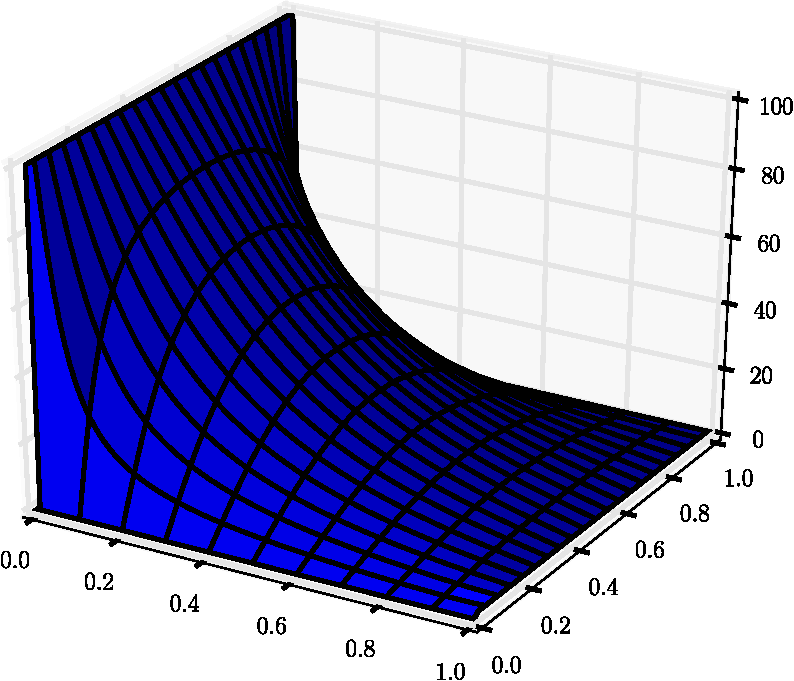
\includegraphics[width=.75\textwidth]{laplace.pdf}
\end{figure}
\end{problem}

\section*{Logical Operations}
Logical operations return arrays of only true or false values.
These arrays are often useful in masking values in other arrays.
\begin{lstlisting}
>>> a = np.random.rand(5,5)
>>> a<.5
array([[ True, False, False,  True, False],
       [ True,  True, False,  True, False],
       [False,  True,  True, False, False],
       [False, False,  True, False,  True],
       [ True, False, False,  True, False]], dtype=bool)
>>> a[a<.5]
array([ 0.46121936,  0.11294639,  0.37868745,  0.23435659,  0.25898226,
        0.09095808,  0.19124312,  0.41124911,  0.09823221,  0.03739077,
        0.08655778])
>>> a[a<.3] = 0
>>> a
array([[ 0.46121936,  0.83080909,  0.5632045 ,  0.        ,  0.59581868],
       [ 0.37868745,  0.        ,  0.54977124,  0.        ,  0.753893  ],
       [ 0.79744663,  0.        ,  0.        ,  0.57981239,  0.95839037],
       [ 0.66512744,  0.63471169,  0.41124911,  0.6466058 ,  0.        ],
       [ 0.        ,  0.50692736,  0.54082953,  0.        ,  0.5173614 ]])
\end{lstlisting}
The comparison operators can all be used like this with arrays.
We can quickly test if all elements of a given axis evaluate to true with \li{np.all}.  Likewise, we can test if any element evaluates to true with \li{np.any}.  
Because of the nature of floating point numbers, it is next to impossible to accurately test the equality of elements of two arrays.
NumPy provides a special function, \li{np.allclose}, to check if two arrays are \emph{almost} the same (or within some specified tolerances).  \emph{Please note that in some rare cases \li{np.allclose(a, b)} will not match \li{np.allclose(b, a)}.}  This is because the equation the function uses for checking closeness is not symmetric ($\abs{a-b} \leq \mbox{atol} + \mbox{rtol}*\abs{b}$).      
\begin{lstlisting}
>>> a = np.ones((5, 5))
>>> np.allclose(a, a+1e-5)
True
>>> np.allclose(a, a+1e-4)
False
\end{lstlisting}
NumPy also allows bitwise operations on arrays using the standard Python bitwise operators: \li{&}, \li{|}, and \li{^}.
They are also available available as NumPy functions: \li{np.bitwise_and}, \li{np.bitwise_or}, and \li{np.bitwise_xor} respectively.
The makes available logical opertators as well: \li{np.logical_and}, \li{np.logical_or}, and \li{np.logical_xor}.


\section*{Saving Arrays}
It is often useful to save an array as a file.
NumPy provides several easy methods for saving and loading array data.
\begin{table*}[h]
\begin{tabular}{l|l}
\hline
\li{np.save(file, arr)} & Save an array to a binary file \\
\li{np.savez(file, *arrs)} & Save multiple arrays to a binary file \\
\li{np.savetxt(file, arr)} & Save an array to a text file \\
\hline
\end{tabular}
\end{table*}

\begin{table*}[h]
\begin{tabular}{l|l}
\hline
\li{np.load(file)} & Load and return an array from a binary file \\
\li{np.loadtxt(file)} & Load and return an array from text file \\
\hline
\end{tabular}
\end{table*}

Let's practice saving an array to a file and loading it again.
Note that, when saving an array, NumPy automatically appends the extension \li{.npy} if it is not already present.
\begin{lstlisting}
a = np.arange(30)
np.save('test_arr', a)
new_a = np.load('test_arr.npy')
np.savez('test_multi', a=a, new_a=new_a)
arrs = np.load('test_multi.npz')
\end{lstlisting}
The variable \li{arrs} points to a dictionary object with the keys \li{a} and \li{new_a} which reference the arrays that have been saved.
The \li{.npz} file extension is the file type used to store multiple arrays.
